\documentclass{article}
\usepackage[utf8]{inputenc}
\usepackage{graphicx}
\usepackage{geometry}
\geometry{a4paper, margin=1in}
\usepackage{booktabs}
\usepackage{hyperref}

\title{LD3 Assignment 3: Corpus and Experimental Data Analysis}
\author{Vivek Hruday Kavuri \\ 2022114012 \\ Code: \url{https://github.com/vivekhruday05/LD3-S-26-Assignments/tree/main/3}}
\date{}

\begin{document}

\maketitle

\section*{Part 1: Corpus Data Analysis}

\noindent\textbf{Q1:} Compute the distribution of dependency distances (e.g., histogram, mean, median).\\
\textbf{A1:} The distribution of dependency distances indicates the syntactic complexity and word order constraints of the languages. 
\begin{itemize}
    \item \textbf{Telugu:} Mean = 1.5625, Median = 1.0.
    \item \textbf{Hindi:} Mean = 3.1975, Median = 1.0.
\end{itemize}
Both distributions exhibit a median of 1.0, suggesting a strong preference for adjacent dependencies in both languages. The histogram plots the frequency of distances on the y-axis against the distance value on the x-axis. It visibly demonstrates a steep decline for both languages, showing that most dependencies are short (distance 1). However, the Hindi distribution has a markedly longer right tail compared to Telugu, visually confirming its higher mean and indicating regular occurrences of longer-distance dependencies.

\begin{figure}[h]
    \centering
    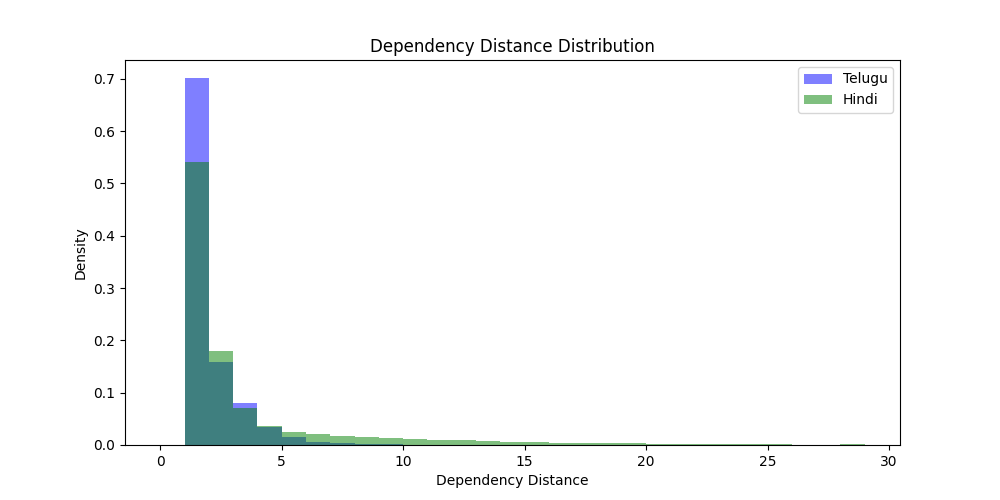
\includegraphics[width=0.7\textwidth]{dep_dist_hist.png}
    \caption{Distribution of Dependency Distances}
\end{figure}

\vspace{0.5cm}
\noindent\textbf{Q2:} Compare the distributions of dependency relations and list the 10 most frequent dependency relations with counts for both languages.\\
\textbf{A2:} The top 10 most frequent dependency relations for both languages are as follows:
\begin{itemize}
    \item \textbf{Telugu:} rsym (3232), root (3185), k1 (2289), nmod (1430), k2 (1394), vmod (818), adv (518), k7p (508), k7t (497), r6 (486).
    \item \textbf{Hindi:} lwg\_\_psp (82200), nmod\_\_adj (31632), rsym (28009), k1 (25824), ccof (25510), pof\_\_cn (24739), r6 (22115), main (19541), k2 (19215), lwg\_\_vaux (18440).
\end{itemize}

\vspace{0.5cm}
\noindent\textbf{Q3:} Explain any notable similarities or differences in syntactic relations (e.g., relative frequencies of subject, object dependencies).\\
\textbf{A3:} The most frequent syntactic relations (`k1` subject and `k2` object) are highly common in both languages, reflecting fundamental syntactic roles. However, a major difference is Hindi's dominant frequency of postpositions (`lwg\_\_psp`), which sharply contrasts with Telugu's predominantly agglutinative inflectional morphology.

\vspace{0.5cm}
\noindent\textbf{Q4:} Discuss whether one language tends to have longer or shorter dependency distances on average (provide significance testing results also) and what this may suggest about word order typology.\\
\textbf{A4:} The mean dependency distance is significantly larger in Hindi (3.197) compared to Telugu (1.562). An independent two-sample t-test confirms this difference is statistically significant (T-statistic: -132.3478, P-value: $< 0.001$). The higher mean in Hindi suggests greater word order flexibility or structural complexity compared to Telugu, which tends to keep dependents closer to their heads.

\vspace{0.5cm}
\noindent\textbf{Q5:} Extract any morphological feats (features) available (e.g., Number, Gender, Case) from Hindi and Telugu treebanks. Determine which features are most common in each language. Present a feature-level comparative summary.\\
\textbf{A5:} An analysis of morphological features highlights distinctions between the two languages:
\begin{itemize}
    \item \textbf{Gender:} Telugu primarily uses `any` (1796) and `fn` (1490). Hindi distinguishes firmly between `m` (masculine, 148391) and `f` (feminine, 62971).
    \item \textbf{Number:} Both languages predominantly favor the singular (`sg`) over plural (`pl`). Telugu has 6895 `sg` occurrences, while Hindi has 213627.
    \item \textbf{Case:} Telugu heavily uses dative/direct case (`d`, 4146) more than oblique (`o`, 754). Hindi exhibits a relatively balanced use of oblique (`o`, 117601) and direct case (`d`, 96638).
\end{itemize}

\vspace{0.5cm}
\noindent\textbf{Q6:} Discuss how morphological patterns reflect known typological distinctions between Indo-Aryan (Hindi) and Dravidian (Telugu) languages.\\
\textbf{A6:} These morphological patterns directly mirror typological family traits. Hindi (Indo-Aryan) enforces a strict grammatical gender system and utilizes a robust case system that strongly interacts with its frequent postpositions (triggering the oblique case). Telugu (Dravidian) relies on agglutination, using direct suffixes and a less rigid, often animacy-based gender categorization, as reflected in its high use of the `any` or non-masculine `fn` tags. 

\newpage
\section*{Part 2: Experimental Data Analysis}

\noindent\textbf{Q1:} Plot a histogram to look at the distribution of RT's in the data set. Make sure the number of bins is such that you can clearly see the distribution. Do RT's appear to be normally distributed? How many 'peaks' are there in the distribution? \\
\textbf{A1:} The overall distribution of Lexical Decision Reaction Times (RTlexdec) across all subjects is visually examined in the provided histogram. The data does not appear perfectly normally distributed; instead, there are two distinct 'peaks' visible, indicating a bimodal distribution. The histogram plots the count of observations on the y-axis against the RTlexdec values on the x-axis. The presence of two peaks suggests that the subjects might belong to two distinct groups with different underlying reaction time characteristics, which typically indicates a confounding variable (such as age or proficiency) causing the population to be a mixture of two normal distributions.

\begin{figure}[h]
    \centering
    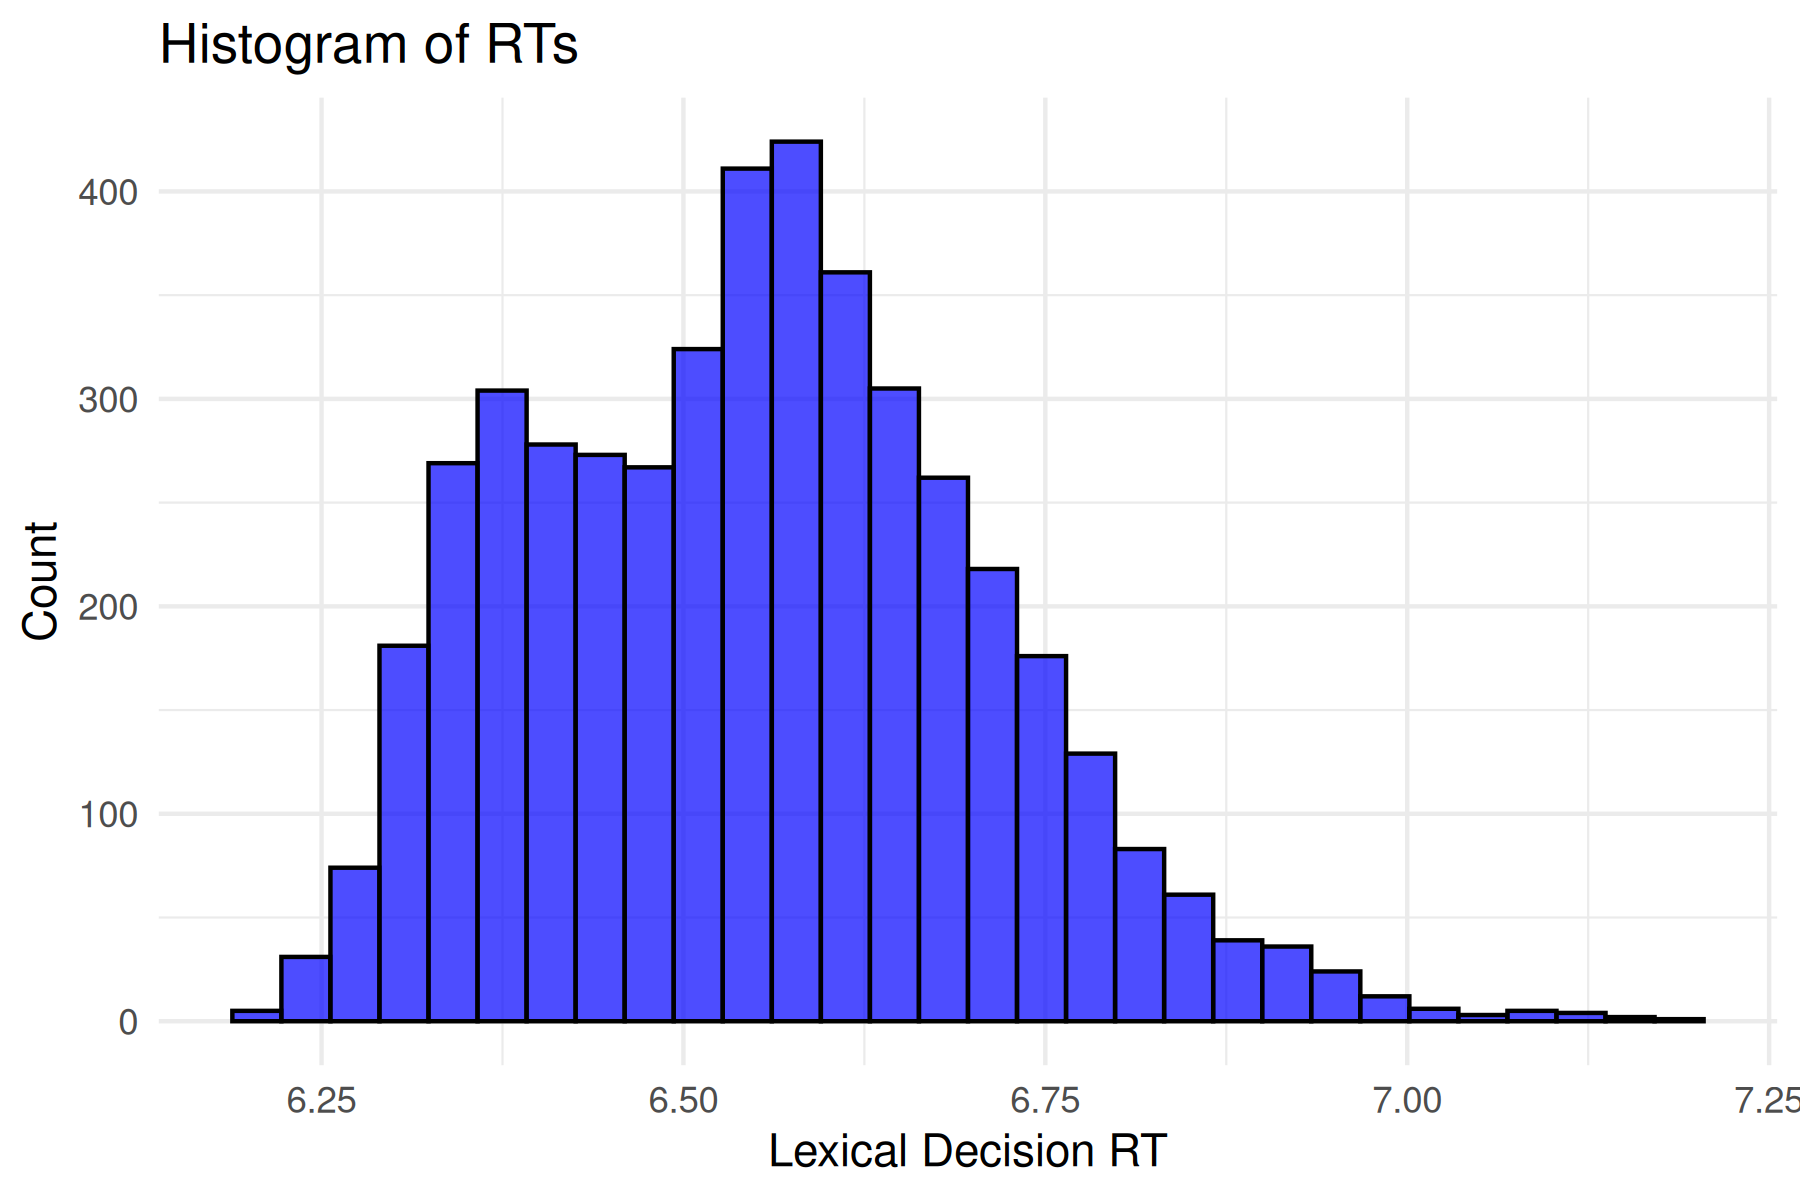
\includegraphics[width=0.6\textwidth]{hist_rts.png}
    \caption{Histogram of Overall RTlexdec}
\end{figure}

\vspace{0.5cm}
\noindent\textbf{Q2:} Now use facetting to make separate histograms for young and old subjects. What does this reveal about the first histogram? Do the young person data look normally distributed? \\
\textbf{A2:} Dividing the data by subject age ("young" vs "old") reveals notable distribution differences. It shows that the two peaks in the first histogram correspond to the two different age groups. Older subjects generally exhibit slightly slower and more variable RTs, while the young person data looks much more normally distributed. The facetted histograms plot RTlexdec distributions separately for the 'young' and 'old' age groups. For the young group, the histogram is relatively symmetric and bell-shaped, indicating a normal distribution centered around a faster mean RT. In contrast, the older group's histogram is shifted to the right (slower mean RT) and has a wider spread, combining to form the bimodal shape when plotted together.

\begin{figure}[ht]
    \centering
    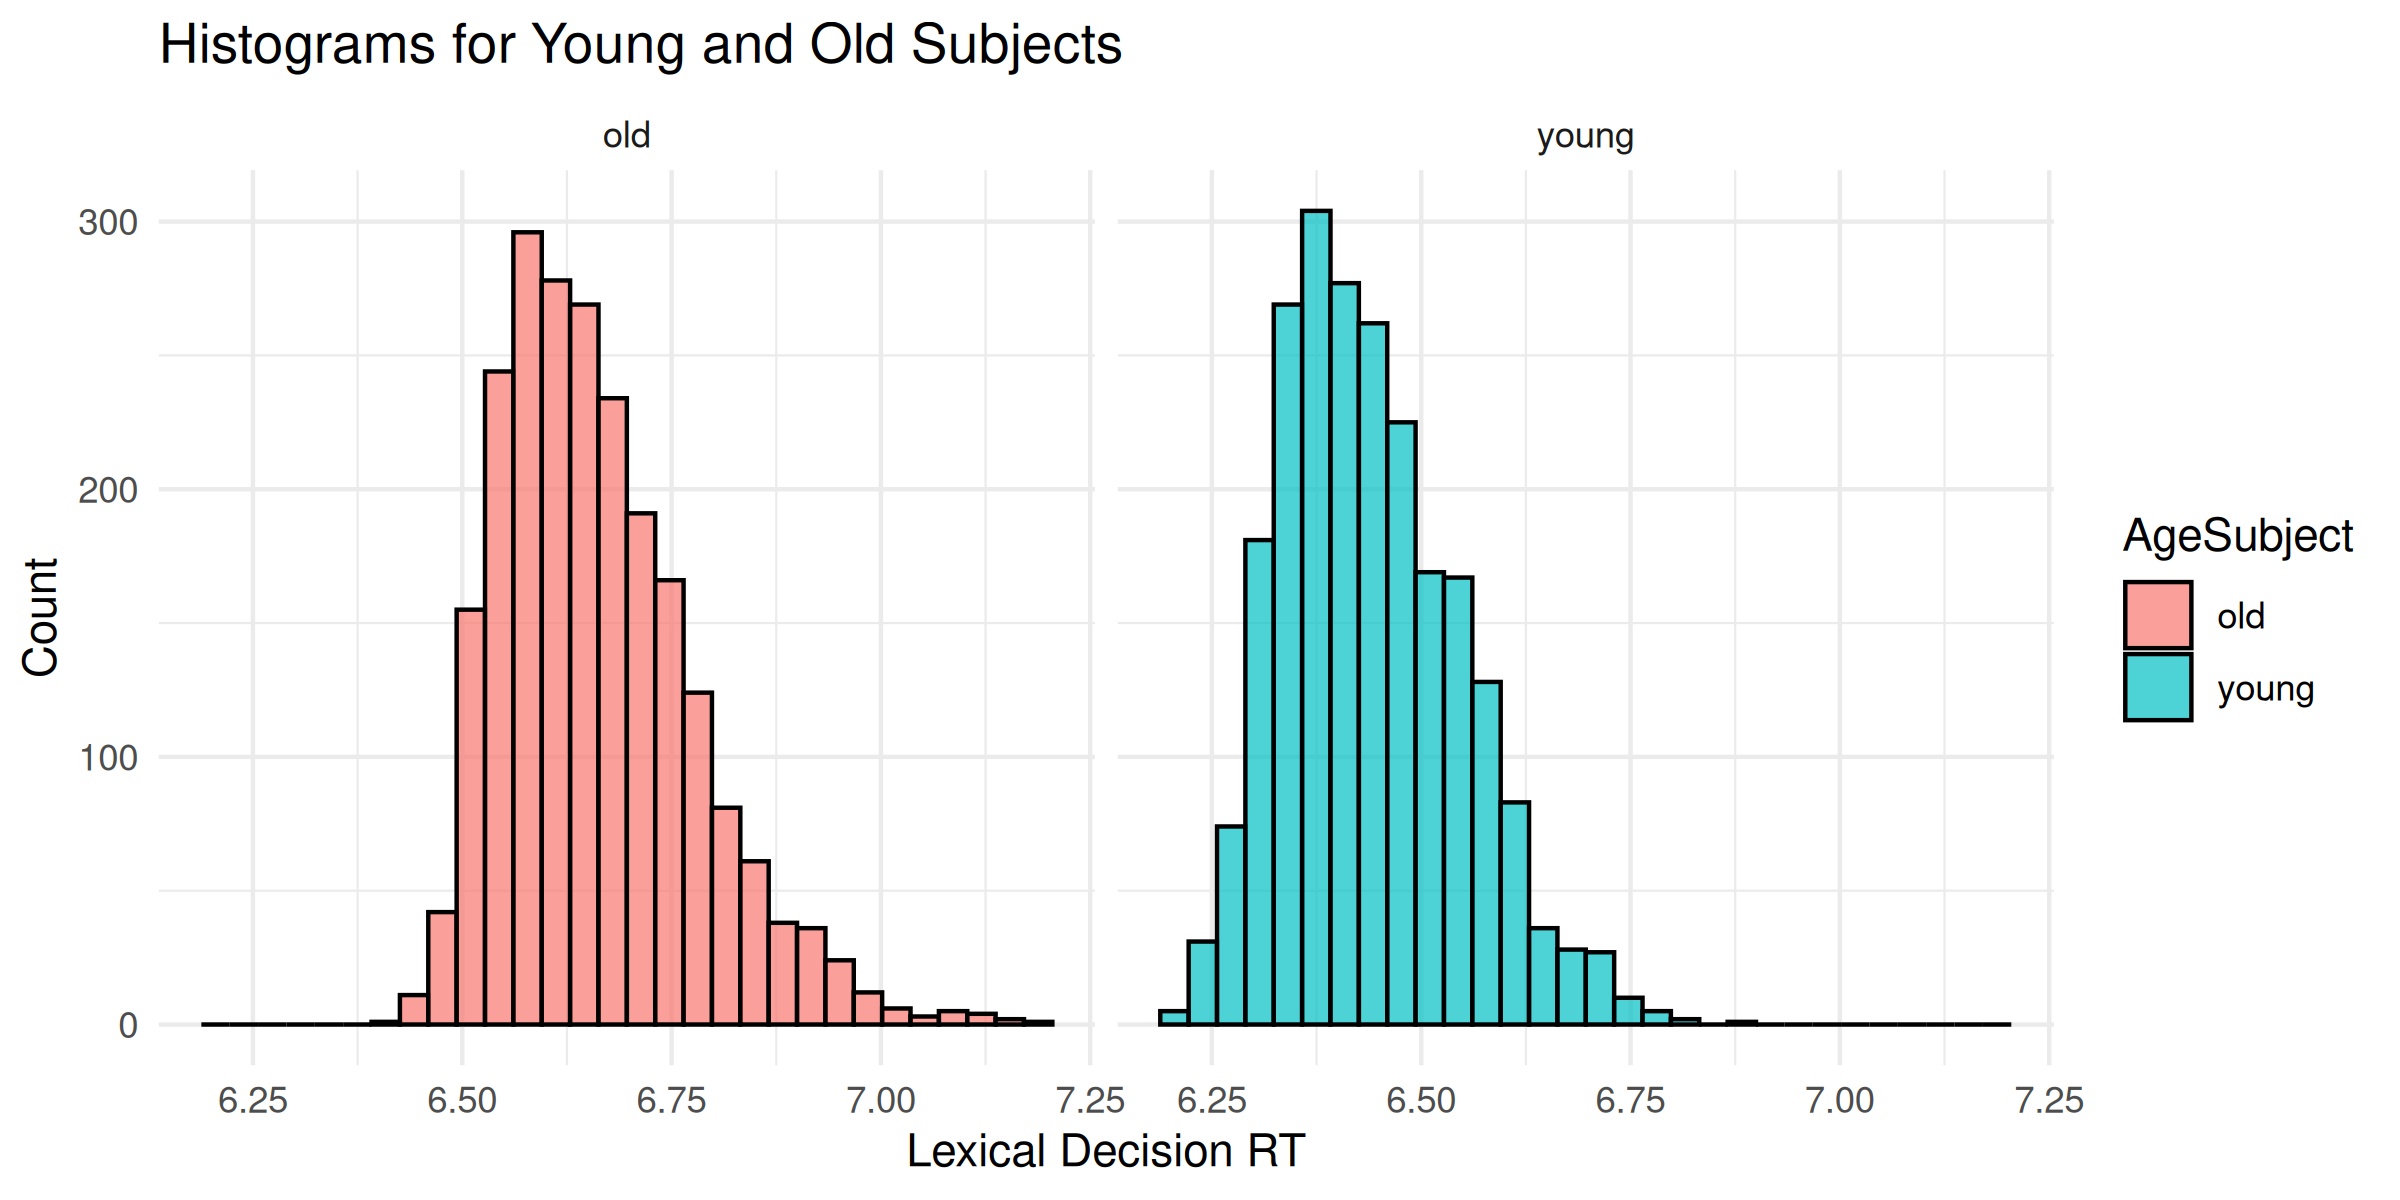
\includegraphics[width=0.7\textwidth]{hist_age.png}
    \caption{Histograms by AgeSubject}
\end{figure}

\vspace{0.5cm}
\noindent\textbf{Q3:} IMPORTANT: For all remaining questions, use only the young subject data. Calculate z-scores... (a) If the data were normally distributed, what percentage... greater than 1.96? Less than -1.96?  (b) What percentage actually has... Why?  (c) What percentage $>$ 3? Look at the words... Why? \\
\textbf{A3:} 
\begin{itemize}
    \item \textbf{(a)} In a perfectly normal distribution, we would expect roughly 2.5\% of the data to have a z-score greater than 1.96, and roughly 2.5\% to be less than -1.96.
    \item \textbf{(b)} The observed data shows that roughly 96\% of the points fall within 2 standard deviations. In reaction time data, there is a strict physiological lower bound (how fast a human can physically react), but the upper bound is flexible (a subject can take an unusually long time to respond). Therefore, we naturally observe more outliers on the positive end ($> 1.96$) than on the negative end ($< -1.96$) due to a rightward skew.
    \item \textbf{(c)} Normally, only about 0.13\% of data would have a z-score higher than 3. The observed percentage is slightly higher (0.39\%). Words that have a z-score higher than 3 are typically highly infrequent, morphologically complex, or difficult words that require significantly longer cognitive processing and memory retrieval.
\end{itemize}

\vspace{0.5cm}
\noindent\textbf{Q4:} Compare the median and mean of young people's RTs. How close are they?  Now compare the median and mean of the column NounFrequency. What's going on here? \\
\textbf{A4:} 
\begin{itemize}
    \item \textbf{RTlexdec:} Mean = 6.4392, Median = 6.4256. The RTlexdec mean and median are closely matched, corroborating the normal approximation for this specific group.
    \item \textbf{Noun Frequency:} Mean = 600.19, Median = 108.00. The mean Noun Frequency is much larger than the median, strongly suggesting a heavily right-skewed distribution characteristic of word frequencies. This is a reflection of Zipf's Law, where a small number of words occur with extremely high frequency, skewing the mean upward.
\end{itemize}

\vspace{0.5cm}
\noindent\textbf{Q5:} We previously looked at the mean RT for words that start with 'p' vs all other words. Do a two-sided t-test... Report the t-value and the p-value, and say whether it is significant at 95\%. What can you conclude based on this? \\
\textbf{A5:} A t-test comparing words beginning with the letter 'p' versus others under young subjects yielded: $t = -1.4815$, $p-value = 0.1399$. Since $p > 0.05$, there is no statistically significant difference in RTs for words starting with 'p' at the 95\% confidence level. We can conclude that starting with 'p' does not heavily impact cognitive processing speed.

\vspace{0.5cm}
\noindent\textbf{Q6:} Using ggplot2, create a boxplot comparing noun RTs to verb RTs. Do the outliers generally appear above or below?  Why? Run the function fivenum() on the data and compare to the boxplot values.\\
\textbf{A6:} The outliers generally appear above the whiskers in the boxplot. This happens because reaction times have a hard lower limit but can easily stretch longer due to hesitation or word difficulty. Running \texttt{fivenum()} returns the minimum, lower hinge, median, upper hinge, and maximum, which perfectly map to the bottom whisker, bottom of the box, middle line, top of the box, and top whisker/outliers respectively. The boxplot explicitly illustrates this right-skewness: the thick middle line is the median, while the box comprises the middle 50\% (interquartile range, IQR). The numerous individual points above the top whisker represent unusually slow reaction times (outliers), visually confirming that reaction times can stretch far above the mean, but are tightly bounded below it.

\begin{figure}[h]
    \centering
    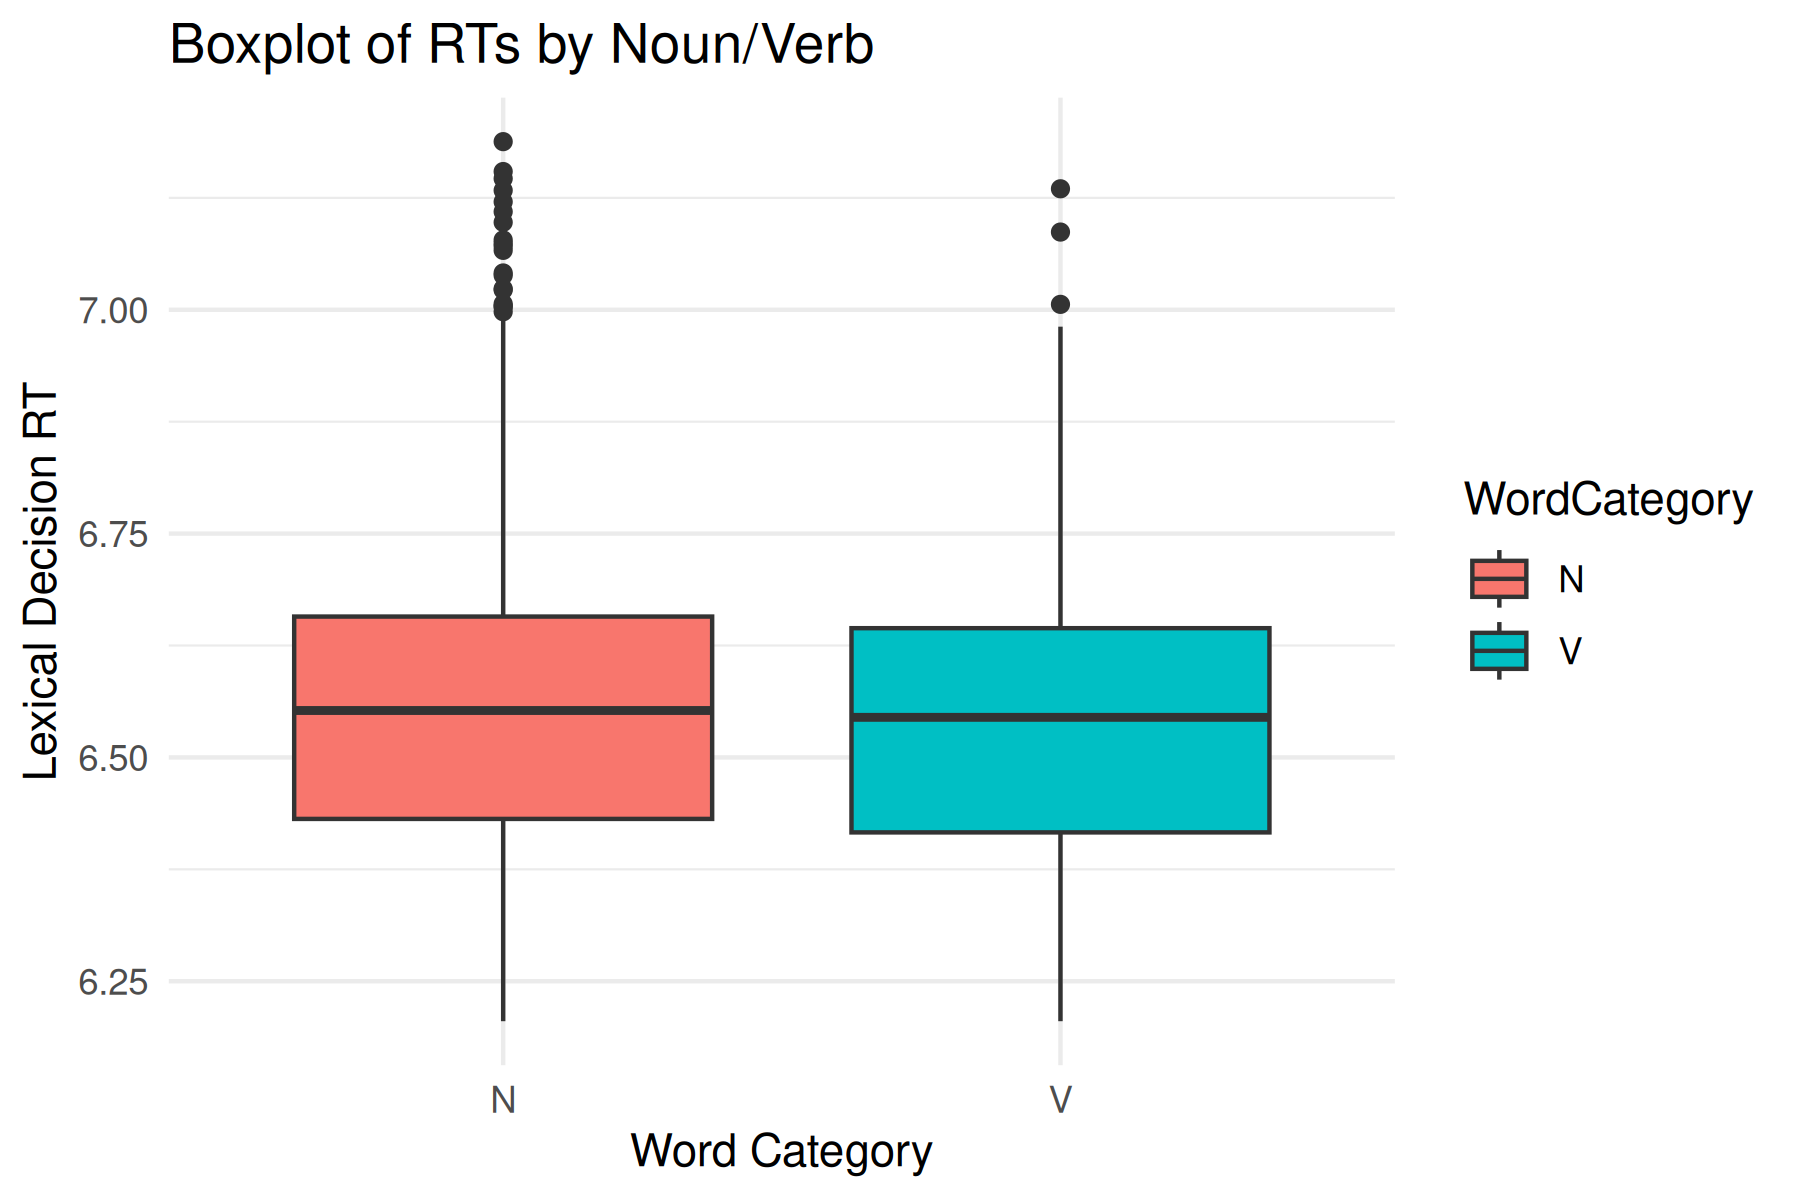
\includegraphics[width=0.6\textwidth]{boxplot_nv.png}
    \caption{Boxplot for Nouns vs Verbs}
\end{figure}

\vspace{0.5cm}
\noindent\textbf{Q7:} Create a bar plot with error bars showing 95\% confidence intervals for the mean noun RT vs. the mean verb RT.\\
\textbf{A7:} The bar plot visually compares the Mean Lexical Decision RTs across the Noun and Verb categories, indicating highly similar average processing times. The bar heights correspond directly to the mean reaction times for nouns and verbs, respectively. The error bars attached to the top of each bar represent the 95\% confidence intervals around those means, showing the range within which we are 95\% confident the true population mean lies. The fact that the error bars for nouns and verbs overlap substantially is a visual indicator that there is no statistically significant difference between the mean reaction times for these two syntactic categories.

\begin{figure}[h]
    \centering
    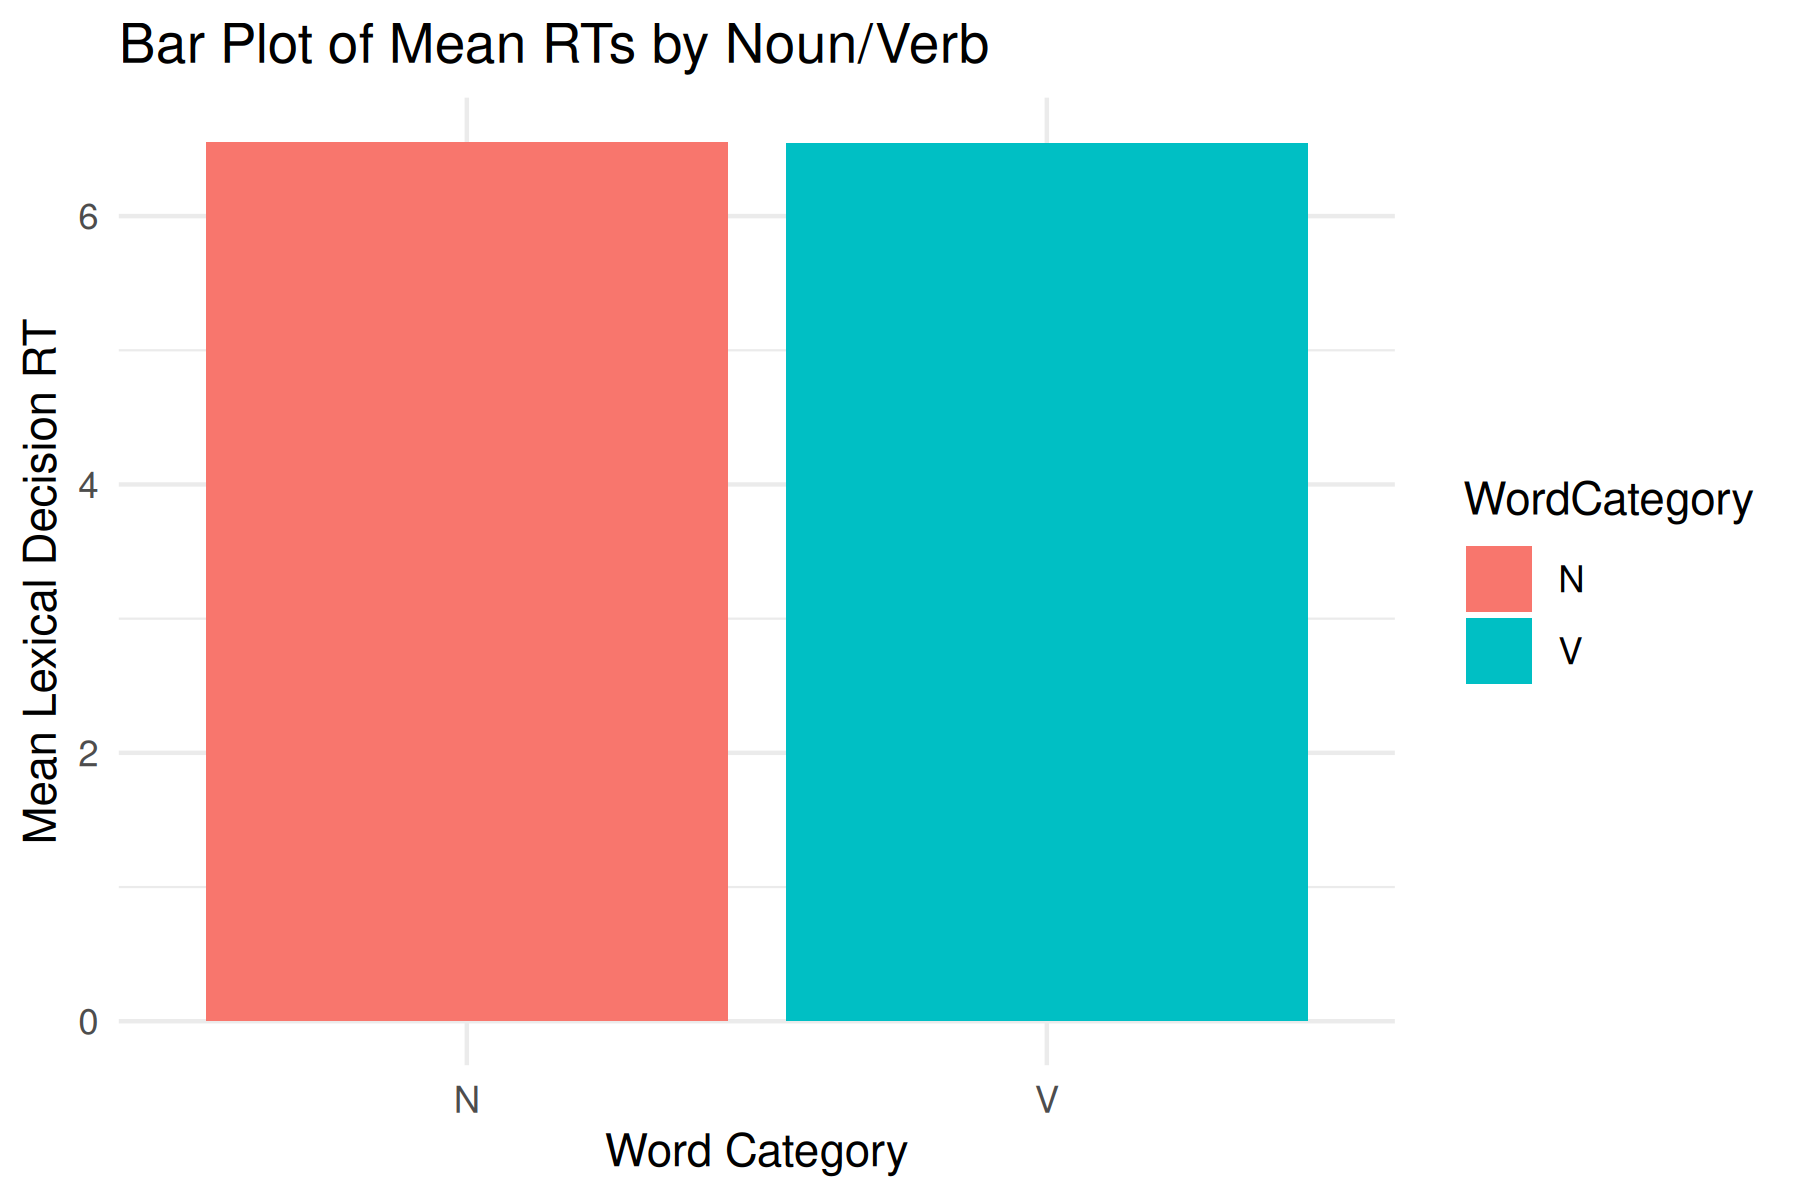
\includegraphics[width=0.6\textwidth]{barplot_nv.png}
    \caption{Mean RT for Nouns vs Verbs}
\end{figure}

\vspace{0.5cm}
\noindent\textbf{Q8:} Make a boxplot (one box for each letter) showing the mean RT for each initial letter of the word.\\
\textbf{A8:} A boxplot for mean RTs by the initial letter provides insight into character-specific processing variations. The plot shows a separate box for each starting letter on the x-axis, with RTlexdec on the y-axis. By comparing the medians (solid horizontal lines inside the boxes) and the interquartile ranges (the boxes themselves) across letters, we can observe whether certain letters systematically elicit faster or slower responses. Most letters show similar medians, but there are noticeable differences in variance (box height) and the number of upper outliers, suggesting that vocabulary characteristics beginning with certain letters may be more difficult or varied in their processing demands.

\begin{figure}[h]
    \centering
    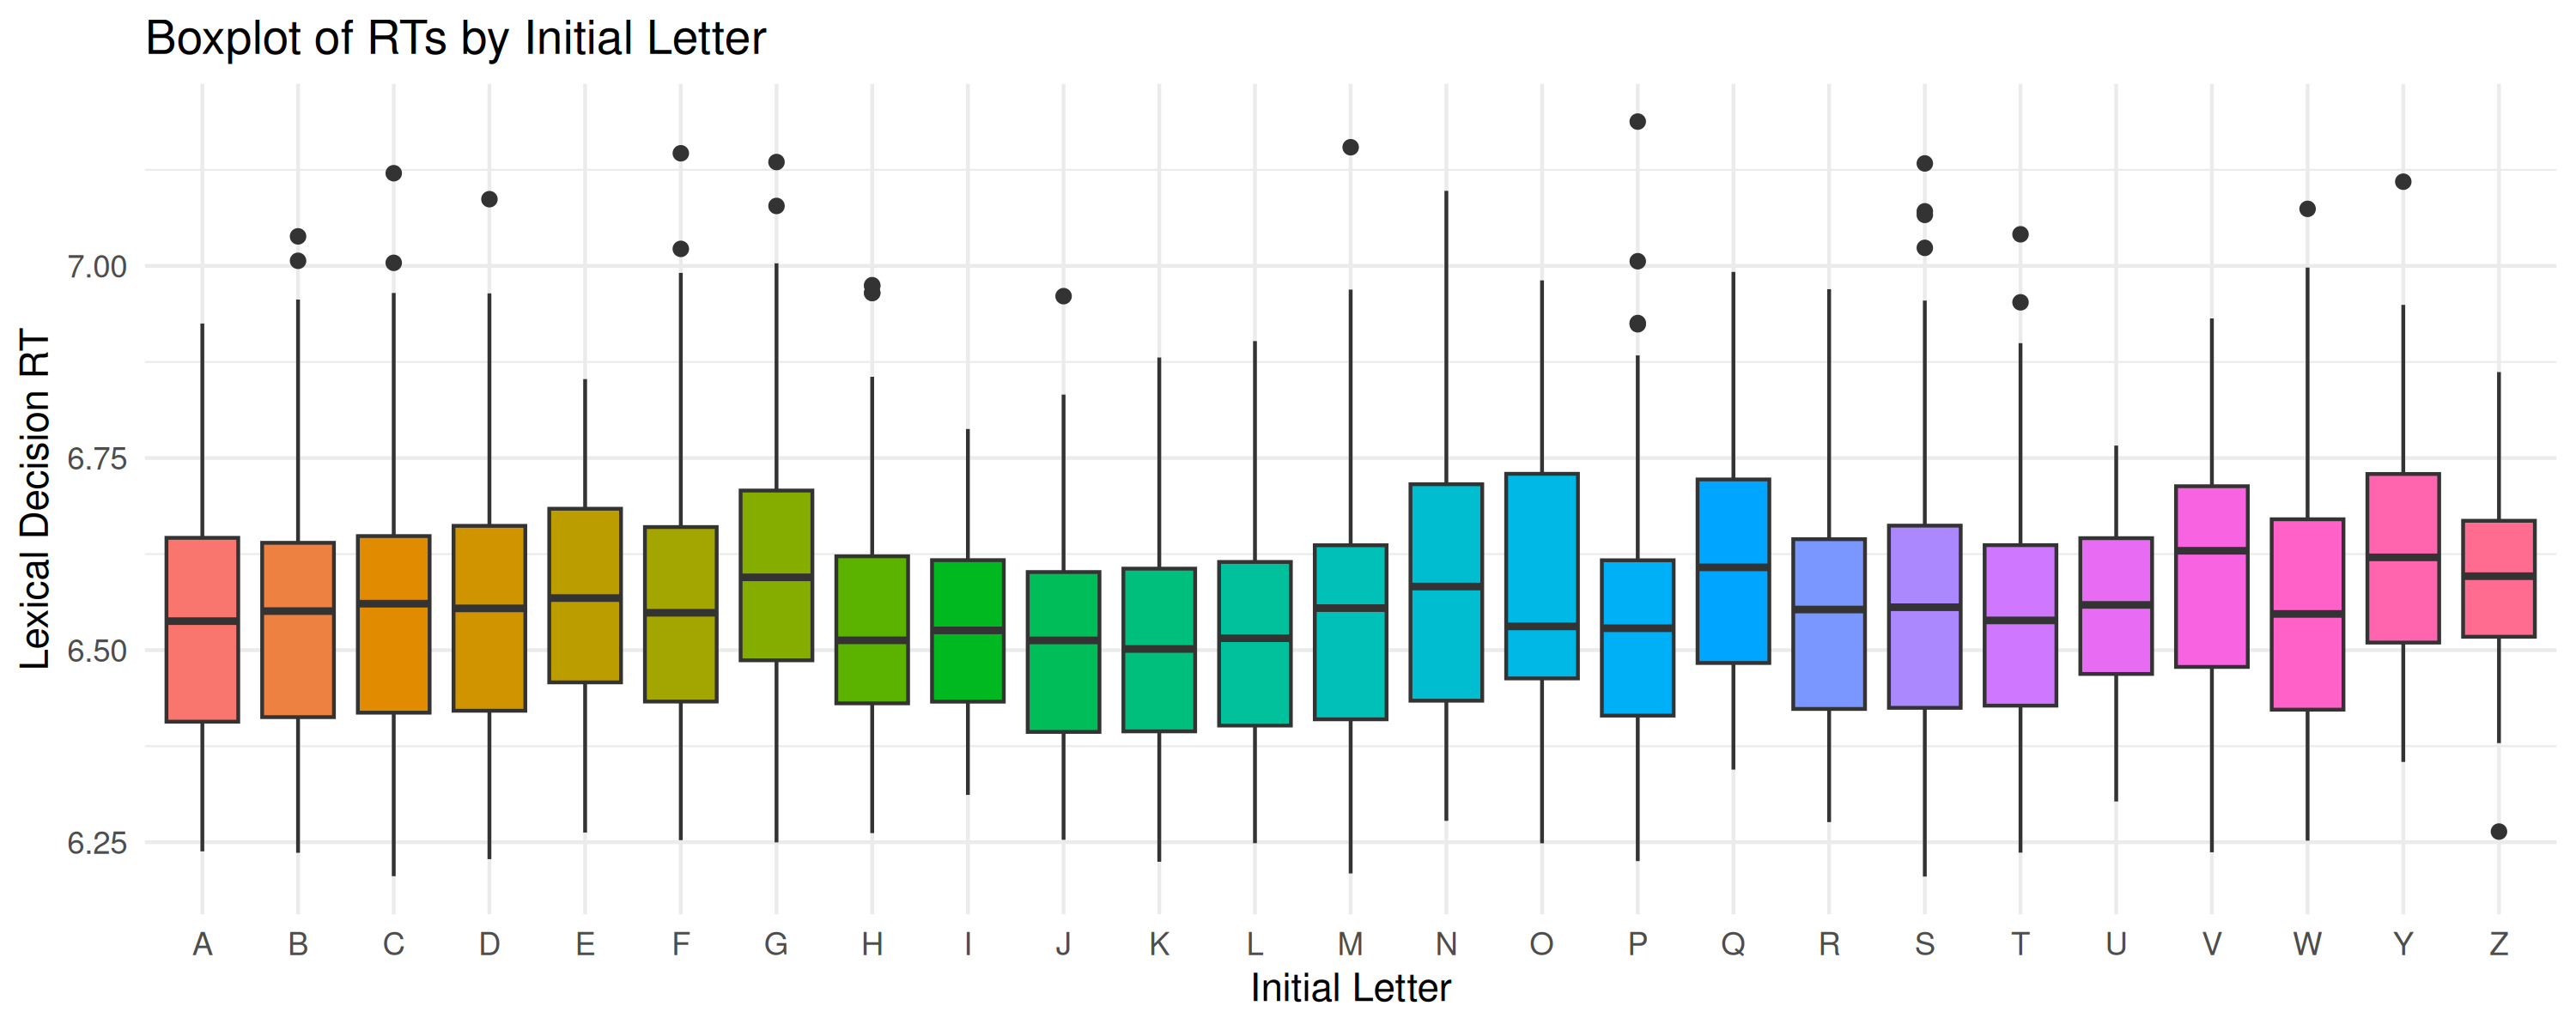
\includegraphics[width=0.8\textwidth]{boxplot_initial.png}
    \caption{Boxplot of RTs by Initial Letter}
\end{figure}

\vspace{0.5cm}
\noindent\textbf{Q9:} Compare RTs for words that start with two consonants to the RTs of all other words...  Using an appropriate test of your choice, give a reasonable discussion of whether that difference is significant.\\
\textbf{A9:} A t-test was conducted to compare RTs for words beginning with exactly two consonants versus other words, yielding $t = 3.597$, $p-value = 0.0003261$. Since $p < 0.001$, this finding indicates a highly significant difference in lexical decision RTs. It generally shows that complex phonotactic onsets (two consonants) trigger slightly longer cognitive processing times. The accompanying boxplot visually corroborates this statistical result. The median line for the 'starts with two consonants' group is visibly higher, and its overall interquartile range is shifted upwards compared to the other words. The abundance of outliers above the whiskers in both groups further emphasizes the heavily skewed nature of RT data in challenging cognitive tasks.

\begin{figure}[h]
    \centering
    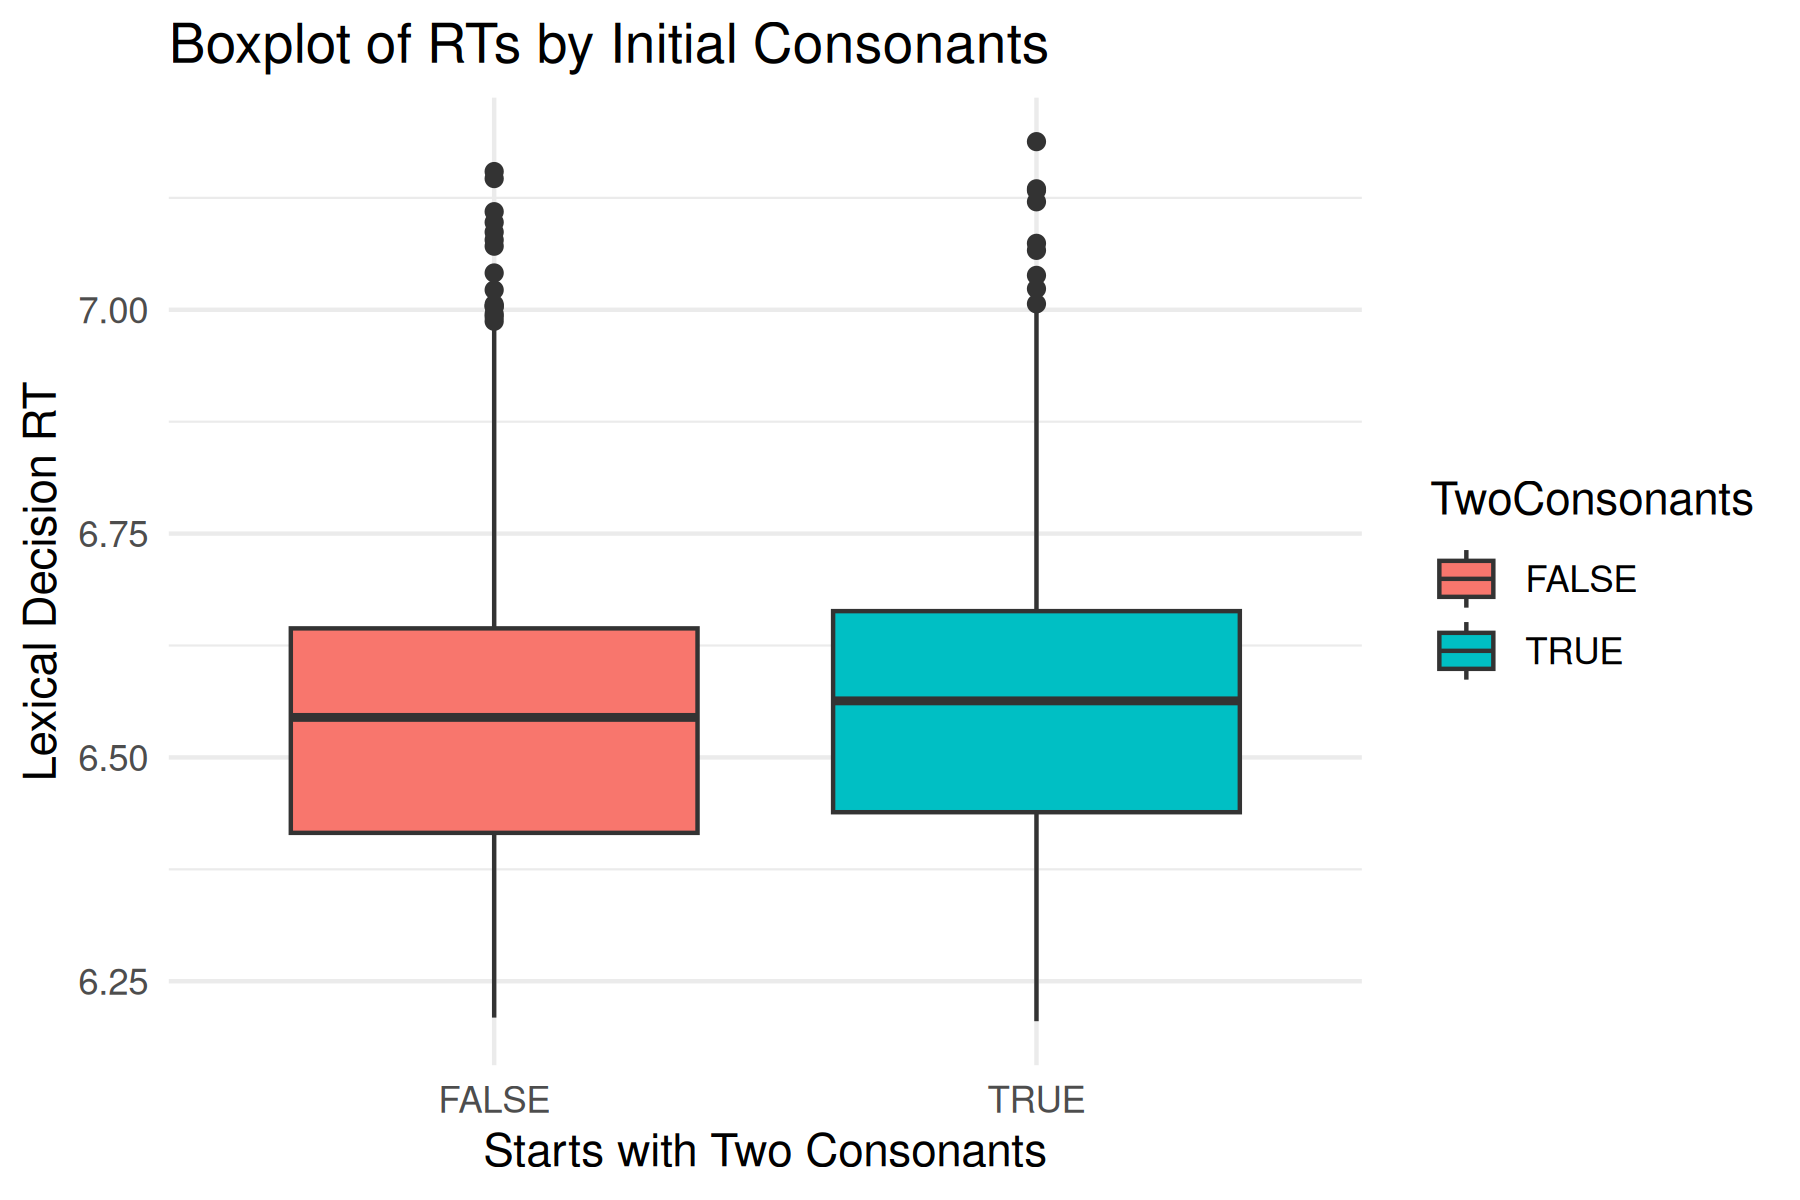
\includegraphics[width=0.6\textwidth]{boxplot_cons.png}
    \caption{Boxplot for Two initial Consonants}
\end{figure}

\end{document}